\documentclass{mm2}
\usepackage{bbm}
\usepackage{bbold}

\newcommand{\mbf}[1]{{\mathbf #1}}
\newcommand{\B}[1]{{\color{blue}#1} }
\newcommand{\vb}[1]{{\tt #1}}

\newcommand{\bu}{{\bf u}}
\newcommand{\bA}{{\bf A}}
\newcommand{\bB}{{\bf B}}
\newcommand{\tr}{{\rm tr}}
\newcommand{\bnabla}{\boldsymbol{\nabla}}

% FILL THIS WITH YOUR CIS USERNAME
\cisid{bzqs27} 
\title{Seismic Waves}

\begin{document}

\begin{abstract}
The purpose of this essay is to analyse the propagation of Seismic waves throughout the Earth. We will be exploring the ray paths between a source and a receiver and using this to gain an understanding of the paths seismic waves take when propagating throughout the earth. When analysing the ray path of individual rays we will consider factors such as travel time and how this information applies in a real-life scenario. For instance, if an earthquake occurs at point A and a Seismic waves is propagated then we would like to know if that effects people at B and how long they have until they will be experiencing the consequences of this effect.
\end{abstract}



\section{Introduction}
Due to the varying depths, density and general physical make-up of the Earth it makes many of the processes that occur within it difficult to model. This certainly includes the propagation of waves throughout the Earth. The largest waves which propagate are those caused by earthquakes, namely Seismic waves. As mentioned in the abstract we will be need to model Seismic waves in order to compute a ray path for each wave. There are two main types of Seismic waves: P (primary) and S (secondary) waves. P waves are longitudinal compression of rocks, and S waves are deformations of rocks in the direction perpendicular to the direction of travel. P and S waves will travel at different speeds and we denote them $V_p$, $V_s$ and $V_p > V_s$. 

Despite there varying speeds and properties, both waves satisfy the same wave equation in 3 dimensions (which as we know is the number of dimensions to the physical universe). The equation is as follows:
\begin{eqnarray}
\frac{1}{V^2}\frac{\partial^2 \phi}{\partial t^2}&=&\bnabla^2\phi\nonumber\\
&=&\frac{\partial^2 \phi}{\partial x^2}+\frac{\partial^2 \phi}{\partial y^2}+
\frac{\partial^2 \phi}{\partial z^2}
\label{eq_wave}
\end{eqnarray}
\section{The Earth's Structure}
The Earth is a mostly solid ball, consisting of the crust near the surface, which is solid and varies between 3 kilometres and 50 kilometres in depth; the mantel, which is also solid and approximately 2850 kilometres thick; the outer core, which is liquid and 2265 kilometres deep and the inner core which is 1215 kilometres deep and made out of solid nickel and other metals.

Our greatest tool in understanding the Earth's structure is the use of waves. The contrast in properties between the solid mantle and the liquid core, which has lower velocity than the overriding mantle makes it worthwhile to use perform seismological studies on the Earth. Throughout any mathematics in the coming essay, we will model the Earth as spherical and use its average radius when using the radius in many calculations.
\section{Ray Theory}
\begin{answer}{1}
% ANSWER QUESTION 1 HERE
It is useful to understand the propagation speed of waves as they propagate through the Earth, as this can give us an idea of the substances through which they are travelling and the geological make-up of the earth. By sending waves from point to point, depending on how quickly they travel we can draw conclusions about the terrain we are analysing.
We will consider how body waves (P and S) propagate through a medium in which the elastic parameters vary dependent on the spatial location, i.e. dependent on where it is the wave is propagating through.
The following should give us an idea of how the propagation speed can be computed.

The use of ray theory simplifies the solving of elastic wave equations, as this requires exhaustive computational effort. Ray theory involves the tracking of an individual point on the wave-front rather than tracking the complete wave-field. Ray theory can be applied to a multitude of problems.

We shall apply ray theory in practical scenarios in order to gain an insight into how Seismic waves propagate through different layers of the Earth, and ultimately we shall use it to gain an understanding on how this affects locations where earthquakes take place and how the surrounding areas will be affected - and how long it will take until the surrounding areas are affected. 

Often however, Ray Theory is not valid - we must assume that the wave travels at a high frequency, otherwise diffraction, scattering and other factors can greatly affect the model and in this case, ray theory is not valid.

Let V denote the propagation speed of the wave, be it a primary or secondary wave. - the propagation speed may be modelled by the same equation as we mentioned earlier. We will assume V to be constant as it represents a propagation speed, thus we must find $\phi$ such that:
\begin{eqnarray}
\frac{1}{V^2}\frac{\partial^2 \phi}{\partial t^2}=\frac{\partial^2 \phi}{\partial x^2}+\frac{\partial^2 \phi}{\partial y^2}+
\frac{\partial^2 \phi}{\partial z^2}.
\label{eq_wave}
\end{eqnarray}

Thus if $V$ is a constant then we may find $\phi$ of the form $\phi = A \exp(-iw(t - {\bf k} \cdot {\bf x}))$ where ${\bf k}$  is a constant vector.

As we know that solutions of the Ordinary Differential Equations of the form 
\begin{eqnarray}
\frac{1}{V^2}\frac{\partial^2 \phi}{\partial t^2}&=&\bnabla^2\phi\nonumber\\
&=&\frac{\partial^2 \phi}{\partial x^2}+\frac{\partial^2 \phi}{\partial y^2}+
\frac{\partial^2 \phi}{\partial z^2}
\label{eq_wave}
\end{eqnarray}
have general solutions of the form 
\begin{eqnarray}
\phi^+_k(x,t) = A\exp(kx -wt)
\phi^-_k(x,t) = A\exp(kx +wt)
\end{eqnarray}
we can assume the solution of the general solution of the prior mentioned wave equation to be of the form $\phi = A \exp(-iw(t - {\bf x} \cdot {\bf k} ))$ where ${\bf k}\cdot {\bf x} = k_1x + k_2y + k_3z$.

We can show that $\phi = A \exp(-iw(t - {\bf k}\cdot {\bf x}))$ is of the correct form as it satisfies the general wave equation in 3 dimensions: \begin{eqnarray}
\frac{1}{V^2}\frac{\partial^2 \phi}{\partial t^2}&=&\bnabla^2\phi\nonumber\\
&=&\frac{\partial^2 \phi}{\partial x^2}+\frac{\partial^2 \phi}{\partial y^2}+
\frac{\partial^2 \phi}{\partial z^2}
\label{eq_wave}
\end{eqnarray}.


To show this we compute the following:
\begin{eqnarray}
\frac{\partial^2\phi}{\partial t^2}&=&\frac{\partial}{\partial t} \left(  \frac{\partial}{\partial t}  \left(  A\exp(-iw(t - {\bf k}\cdot {\bf x} ))  \right) \right)\\ &=&  \frac{\partial}{\partial t} \left( -iwA \exp(-iw(t - {\bf k}\cdot {\bf x} ))\right)\\ &=& -Aw^2 \exp(-iw(t - {\bf k}\cdot {\bf x} ))\\
\end{eqnarray}

\begin{eqnarray}
\frac{\partial^2\phi}{\partial x^2}&=&\frac{\partial}{\partial x} \left(  \frac{\partial}{\partial x}  \left(  A\exp(-iw(t - {\bf k}\cdot {\bf x}))  \right) \right)\\ &=&  \frac{\partial}{\partial x} \left( iwk_1A \exp(-iw(t - {\bf k}\cdot {\bf x} ))\right)\\ &=& -Aw^2k_1^2 \exp(-iw(t - {\bf k}\cdot {\bf x} ))\\
\end{eqnarray}.

\begin{eqnarray}
\frac{\partial^2\phi}{\partial y^2}&=&\frac{\partial}{\partial y} \left(  \frac{\partial}{\partial y}  \left(  A\exp(-iw(t - {\bf k}\cdot {\bf x} ))  \right) \right)\\ &=&  \frac{\partial}{\partial y} \left( iwk_2A \exp(-iw(t - {\bf k}\cdot {\bf x} ))\right)\\ &=& -Aw^2k_2^2 \exp(-iw(t - {\bf k}\cdot {\bf x}))\\
\end{eqnarray}.

\begin{eqnarray}
\frac{\partial^2\phi}{\partial z^2}&=&\frac{\partial}{\partial z} \left(  \frac{\partial}{\partial z}  \left(  A\exp(-iw(t - {\bf k}\cdot {\bf x}))  \right) \right)\\ &=&  \frac{\partial}{\partial z} \left( iwk_3A \exp(-iw(t - {\bf k}\cdot {\bf x} ))\right)\\ &=& -Aw^2k_3^2 \exp(-iw(t - {\bf k}\cdot {\bf x} ))\\
\end{eqnarray}.
\end{answer}

From the relation \begin{eqnarray}
\frac{1}{V^2}\frac{\partial^2 \phi}{\partial t^2}=\frac{\partial^2 \phi}{\partial x^2}+\frac{\partial^2 \phi}{\partial y^2}+
\frac{\partial^2 \phi}{\partial z^2}.
\label{eq_wave}
\end{eqnarray} we know the following

\begin{eqnarray}
\frac{1}{V^2}\left(-Aw^2 \exp(-iw(t - {\bf k}\cdot {\bf x} ))\right) = -Aw^2k_1^2 \exp(-iw(t - {\bf k}\cdot {\bf x} ))\\ -Aw^2k_2^2 \exp(-iw(t - {\bf k}\cdot {\bf x}))\\ -Aw^2k_3^2 \exp(-iw(t - {\bf k}\cdot {\bf x} ))
\end{eqnarray}.

If we divide both the left and right hand side by $(-Aw^2)$ then we arrive at:
\begin{eqnarray}
\Longrightarrow \frac{1}{V^2}\left(\exp(-iw(t - {\bf k}\cdot {\bf x} ))\right) &=& (k_1^2 + k_2^2 + k_3^2))\left(\exp(-iw(t - {\bf k}\cdot {\bf x} ))\right)\\ &=& \mid \mid k \mid \mid {^2} \exp(-iw(t - {\bf k}\cdot {\bf x}))
\end{eqnarray}

If we divide both the left and right hand side by $\exp(-iw(t - {\bf k}\cdot {\bf x} ))$ then we arrive at:
\begin{eqnarray}
\Longrightarrow \frac{1}{V^2} &=& \mid \mid k \mid \mid {^2}
\end{eqnarray}

Simply by multiplying both sides by $\frac{V^2}{\mid \mid k \mid \mid {^2}}$ and then square-rooting both sides we arrive at:
\begin{eqnarray}
\Longrightarrow V = \frac{1}{\mid \mid k \mid \mid}
\end{eqnarray}

This confirms any solution of $ \frac{1}{V^2}\frac{\partial^2 \phi}{\partial t^2}=\frac{\partial^2 \phi}{\partial x^2}+\frac{\partial^2 \phi}{\partial y^2}+
\frac{\partial^2 \phi}{\partial z^2}$ is of the form $\phi = A \exp(-iw(t - {\bf k}\cdot {\bf x} ))$ - where $V$ is constant. 

In order to confirm that $V$ is indeed the speed of the wave we can perform dimensional analysis on the general wave equation (for primary and secondary waves), $\frac{1}{V^2}\frac{\partial^2 \phi}{\partial t^2} = \nabla^2\phi$.
As 
\begin{eqnarray}
\frac{1}{V^2} \frac{\partial^2 \phi}{\partial t^2} = \nabla^2 \phi
\end{eqnarray}
we can replace each of these with their units and the equality will still hold - for clarity:
$\nabla$ represents the rate of change of a distance so its unit is $\frac{1}{m (metres)}$
$\phi$ is a function providing a distance so its unit is $m$ (metres).
$t$ represents time and its unit is seconds.
\begin{eqnarray}
\Rightarrow \frac{1}{V_{units}^2} \frac{m}{s^2} = \frac{1}{m^2} \cdot m\\
\Rightarrow \frac{1}{V_{units}^2}  = \frac{1}{m^2} \cdot m \cdot \frac{s^2}{m}\\
\Rightarrow \frac{1}{V_{units}^2}  = \frac{s^2}{m^2}\\
\Rightarrow V_{units}^2  = \frac{m^2}{s^2}\\
\Rightarrow V_{units} = \frac{m}{s}\\
\end{eqnarray}

The unit $\frac{m}{s}$ or $ms^{-1}$ is the unit consistent with a speed and verifies to us that V represents the propagation speed.












\bigskip
\begin{answer}{2}
% ANSWER QUESTION 2 HERE
However, the above general solution would not be a very precise approximation in a real-life scenario, this is because $V$ is a function of the position as the speed will vary dependent on the position as the properties of the rock vary dependent on where in the Earth the wave is propagating - this may be due to density of the substance through which is is flowing and various other factors.
\begin{figure}
\centering
  \includegraphics[width=9cm]{figures/SpeedDepth.png}
  \caption{The seeds of primary and secondary waves variation with depth.}
  \label{fig:speeddepth1}
\end{figure}

Clearly we can see from the above figure that as the depth at which the wave propagates fluctuates so does the propagation speed of the wave - this suggests there may be superior (but more complicated) method of modelling the Seismic waves in question.

The period of the wave we modelled above was $T=\frac{2 \pi}{w}$. As we are now aware $V$ varies with time, however, if the variation in $V$ is very small ((from Figure 1) we see this could be a period when the wave is propagating at a relatively consistent depth in the Earth) then we can compute distances of the order of the wavelength $\lambda = VT$, these solutions will be similar to the form of $\phi$ in Ray Paths however, rather than having a constant $A$ and the product of constant vectors ${\bf k} \cdot {\bf x} = k_1x + k_2y + k_3x$ we instead use real function $A(\bf x)$ and $T(bf x)$ in order to include the variation of the waves velocity.

We will compute the result of $\phi = A{\bf x} \exp(-iw(t + T({\bf x})))$ in the general wave equation $\left( \frac{1}{V^2}\frac{\partial^2 \phi}{\partial t^2}=\frac{\partial^2 \phi}{\partial x^2}+\frac{\partial^2 \phi}{\partial y^2}+
\frac{\partial^2 \phi}{\partial z^2}\right)$:

Here I will denote the following for ease of typing:
$A({\bf x})$ will be written as $A$,
$T({\bf x})$ will be written as $T$.

Substituting $\phi = A\exp(-iw(t + T))$ into $\left( \frac{1}{V^2}\frac{\partial^2 \phi}{\partial t^2}=\frac{\partial^2 \phi}{\partial x^2}+\frac{\partial^2 \phi}{\partial y^2}+
\frac{\partial^2 \phi}{\partial z^2}\right)$ gives the following:
\begin{eqnarray}
\frac{\partial ^2 \phi}{\partial t^2} &=& \frac{\partial}{\partial t} \left( \frac{\partial}{\partial t} \left( A\exp(-iw(t + T)) \right) \right)\\ &=& left( \frac{\partial}{\partial t} \left( -iAw\exp(-iw(t + T)) \right)\\ &=&  A(-iw)^2\exp(-iw(t + T))\\ &=&  -Aw^2\exp(-iw(t + T)) 
\end{eqnarray}

\begin{eqnarray}
\frac{\partial ^2 \phi}{\partial x^2} &=& \frac{\partial}{\partial x} \left( \frac{\partial}{\partial x} \left( A\exp(-iw(t + T)) \right) \right)\\  &=& \frac{\partial}{\partial x}\left( \frac{\partial}{\partial x}\left(A\right)\exp(-iw(t + T)) + A(-iw)\frac{\partial}{\partial x}(T)\exp(-iw(t + T))\right)\\ &=& \frac{\partial^2}{\partial x^2}\left(A\right)\exp(-iw(t + T)) - iw\frac{\partial}{\partial x}(A)\frac{\partial}{\partial x}(T)\exp(-iw(t + T))\\ &-& iw\left(\frac{\partial}{\partial x}\left(A\right)\frac{\partial}{\partial x}\left(T\right) + A \frac{\partial^2}{\partial x^2}\left(T\right)\right)\exp(-iw(t + T))\\ &+& ((iw)^2 \frac{\partial}{\partial x}(T)A\frac{\partial}{\partial x}(T))\exp(-iw(t + T)) \\ \\
&=& (\frac{\partial^2}{\partial x^2}(A) -iw\frac{\partial}{\partial x} T \frac{\partial}{\partial x} A-iw \frac{\partial}{\partial x}A \frac{\partial}{\partial x}T - iwA\frac{\partial^2}{\partial x^2}T\\ &-& w^2 \frac{\partial}{\partial x}TA\frac{\partial}{\partial x}T)\exp(-iw(t + T)) \\
&=&(\frac{\partial^2}{\partial x^2} A - A \cdot w^2 \cdot \frac{\partial }{\partial x}T \cdot \frac{\partial}{\partial x}T)\\ &+& i (-2w\frac{\partial }{\partial x}A\frac{\partial}{\partial x}T-wA\frac{\partial^2}{\partial x^2}T))\exp(-iw(t + T))
\end{eqnarray}

If we follow identical procedures (replacing $x$ with $y$ and then $z$) then we achieve the following results analogously:

\begin{eqnarray}
\frac{\partial ^2 \phi}{\partial y^2} &=& (\frac{\partial^2}{\partial y^2} A - A \cdot w^2 \cdot \frac{\partial }{\partial y}T \cdot \frac{\partial}{\partial y}T)\\ &+& i (-2w\frac{\partial }{\partial y}A\frac{\partial}{\partial y}T-wA\frac{\partial^2}{\partial y^2}T))\exp(-iw(t + T))
\end{eqnarray}

\begin{eqnarray}
\frac{\partial ^2 \phi}{\partial z^2} &=& (\frac{\partial^2}{\partial z^2} A - A \cdot w^2 \cdot \frac{\partial }{\partial z}T \cdot \frac{\partial}{\partial z}T)\\ &+& i (-2w\frac{\partial }{\partial z}A\frac{\partial}{\partial z}T-wA\frac{\partial^2}{\partial z^2}T))\exp(-iw(t + T))
\end{eqnarray}

I refer back to the commonly used wave equation thus far:
\begin{eqnarray}
\frac{1}{V^2}\frac{\partial^2 \phi}{\partial t^2}=\frac{\partial^2 \phi}{\partial x^2}+\frac{\partial^2 \phi}{\partial y^2}+
\frac{\partial^2 \phi}{\partial z^2}.
\label{eq_wave}
\end{eqnarray}

By employing this relationship once more we can arrive at the followng equality:
\begin{eqnarray}
\frac{1}{V^2}\frac{\partial^2 \phi}{\partial t^2}&=&\frac{\partial^2 \phi}{\partial x^2}+\frac{\partial^2 \phi}{\partial y^2}+
\frac{\partial^2 \phi}{\partial z^2}\\
&=& (\frac{\partial^2}{\partial x^2} A - A \cdot w^2 \cdot \frac{\partial }{\partial x}T \cdot \frac{\partial}{\partial x}T)\\ &+& i (-2w\frac{\partial }{\partial x}A\frac{\partial}{\partial x}T-wA\frac{\partial^2}{\partial x^2}T))\exp(-iw(t + T))\\ &+& (\frac{\partial^2}{\partial y^2} A - A \cdot w^2 \cdot \frac{\partial }{\partial y}T \cdot \frac{\partial}{\partial y}T)\\ &+& i (-2w\frac{\partial }{\partial y}A\frac{\partial}{\partial y}T-wA\frac{\partial^2}{\partial y^2}T))\exp(-iw(t + T))\\ &+& (\frac{\partial^2}{\partial z^2} A - A \cdot w^2 \cdot \frac{\partial }{\partial z}T \cdot \frac{\partial}{\partial z}T)\\ &+& i (-2w\frac{\partial }{\partial z}A\frac{\partial}{\partial z}T-wA\frac{\partial^2}{\partial z^2}T))\exp(-iw(t + T))\\
&=& ((\frac{\partial^2}{\partial x^2} + \frac{\partial^2}{\partial y^2} + \frac{\partial^2}{\partial z^2}) A - A \cdot w^2 \cdot (\frac{\partial }{\partial x} + \frac{\partial}{\partial y} + \frac{\partial}{\partial z}) T\\  &\cdot& (\frac{\partial}{\partial x} + \frac{\partial}{\partial y} + \frac{\partial}{\partial z})T) + i (-2w(\frac{\partial }{\partial x} + \frac{\partial }{\partial y} + \frac{\partial }{\partial z})A(\frac{\partial }{\partial x} + \frac{\partial }{\partial y} + \frac{\partial }{\partial z})T\\ &-& wA (\frac{\partial^2 }{\partial x^2} + \frac{\partial^2}{\partial y^2} + \frac{\partial^2}{\partial z^2}T))\cdot  \exp(-iw(t + T))\\ &=& (({\bf \nabla^2}) A - A \cdot w^2 \cdot ({\bf \nabla}) T  \cdot ({\bf \nabla})T) + i (-2w({\bf \nabla})A({\bf \nabla})T - wA ({\bf \nabla^2}T)) \\ &\cdot&  \exp(-iw(t + T))
\end{eqnarray}

From here we see that the right hand side of the equality, is a complex equation modelling our wave. In order to gain a further insight into the properties of the wave we can equate the real and complex parts of both sides of the equation to result in the following equalities.

This results from equating real parts from both sides.
\begin{eqnarray}
{\bf \nabla^2} A - A \cdot w^2 \cdot {\bf \nabla} T  \cdot {\bf \nabla}T=  -\frac{w^2A}{V^2}
\end{eqnarray}

This results from equating complex parts from both sides.
\begin{eqnarray}
-2w{\bf \nabla} A {\bf \nabla} T - w A {\bf \nabla^2} T =0\\
\Longrightarrow 2w{\bf \nabla} A {\bf \nabla} T + w A {\bf \nabla^2} T =0
\end{eqnarray}

\begin{align}
2\omega \bnabla A \cdot \bnabla T+\omega A \bnabla^2T &=0\,,
\label{eq_AT2a}
\\[1ex]
\bnabla^2A-\omega^2A \bnabla T\cdot\bnabla T
&=-\frac{\omega^2}{V^2}A\,.
\label{eq_AT2b}
\end{align}

This provides us with interesting information about the nature of the functions involved in the wave equation, as well as how their rate of change differs in different dimensions.

Dividing the equation involving the reals by $-A\omega^2$ we obtain
\begin{eqnarray}
-\frac{\bnabla^2A}{A\omega^2}+|\bnabla T|^2
=\frac{1}{V^2}.
\label{eq_AT2c}
\end{eqnarray}
We assume that $V$ changes
very little over a distance of the wavelength $\lambda$. 
Using a Taylor expansion, we can write
\begin{eqnarray}
\frac{{\rm d}^2A(x)}{{\rm d}x^2}\approx \frac{A(x+{\rm d}x)+A(x-{\rm d}x)-2A(x)}{{\rm d}x^2}\,,
\end{eqnarray}
and take ${\rm d}x=\lambda$ so that
\begin{eqnarray}
-\frac{\bnabla^2A}{A\omega^2}&\approx& 
\frac{A(x+{\rm d}x)+A(x-{\rm d}x)-2A(x)}{\lambda^2}\frac{\tau^2}{A(x) 4\pi^2}\nonumber\\
&=&\frac{A(x+{\rm d}x)+A(x-{\rm d}x)-2A(x)}{A(x)}\frac{1}{4\pi^2V^2}\ll\frac{1}{V^2}.
\end{eqnarray}
where $\tau$ is the period of the wave. We use the fact that 
$V=\lambda/\tau$ and we can neglect the first term in (\ref{eq_AT2c})
if $A$ is nearly constant over a distance ${\rm d}x=\lambda$. Then (\ref{eq_AT2c})
simplifies to
\begin{eqnarray}
|\bnabla T|^2
=\frac{1}{V^2}.
\label{eq_eikonala}
\end{eqnarray}

We can simplify this equation to $\mid {\bf \nabla} T \mid ^2 = U^2$ which is referred to as the eikonal equation, where $U$ is the factor 'slowness', $U$ equates to $U = slowness = \frac{1}{V}$.

The transport equation is given by the the equating of complex parts, this is $2w{\bf \nabla} A {\bf \nabla} T + w A {\bf \nabla^2} T =0$ and when divided through by $\omega$ is:



\begin{eqnarray}
2 \bnabla A \cdot \bnabla T+ A \bnabla^2T &=0\,,
\end{eqnarray}

which is the transport equation. The transport equation can be and is often used to compute the amplitude of propagating waves. Also, substitution of the appropriate general S-wave vector into elastic wave equation for an S-wave leads to identical expressions for the eikonal and transport equations. Thus, they are valid for any high-frequency body wave.

\end{answer}


where $T({\bf x})$ is a function providing a constant that defines surfaces called wave-fronts ${\bf \nabla} T({\bf x})$ defines raypaths. The unit of $T({\bf x})$  is time and it represents the time reqired by the wavefront to travel from a point to a point $\bf x$, as mentioned earlier this can be very useful when dealing with earthquakes as in the case of a disaster it offers potential victims a chance to prepare themselves - as well as many other benefits.

If we denote $s$ as the arc length parameter along a ray and $r$ as the position vector, then $\frac{dr}{ds} = \frac{\nabla T}{U}$.

The rate of change of traveltime along the path is simply defined by the slowness, so $\frac{dt}{ds} = U$.

If we take the gradient of both sides, then $\frac{d{\bf \nabla}T}{ds} = {\bf \nabla} U$ noting the commutation of $\frac{d}{ds}$ and ${\bf \nabla}$.

From before, $\nabla T = U \frac{dr}{ds}$, combining this with $\frac{d{\bf \nabla}T}{ds} = {\bf \nabla} U$ we arrive at $\frac{d}{ds} \left[U \frac{dr}{ds}\right] = \nabla U$ which is the kinematic ray equation and describes the trajectory of ray paths in slightly varying isotropic (this means its physical property doesn't differ when measure in different directions) media.

\begin{figure}[ht]
    \centering
  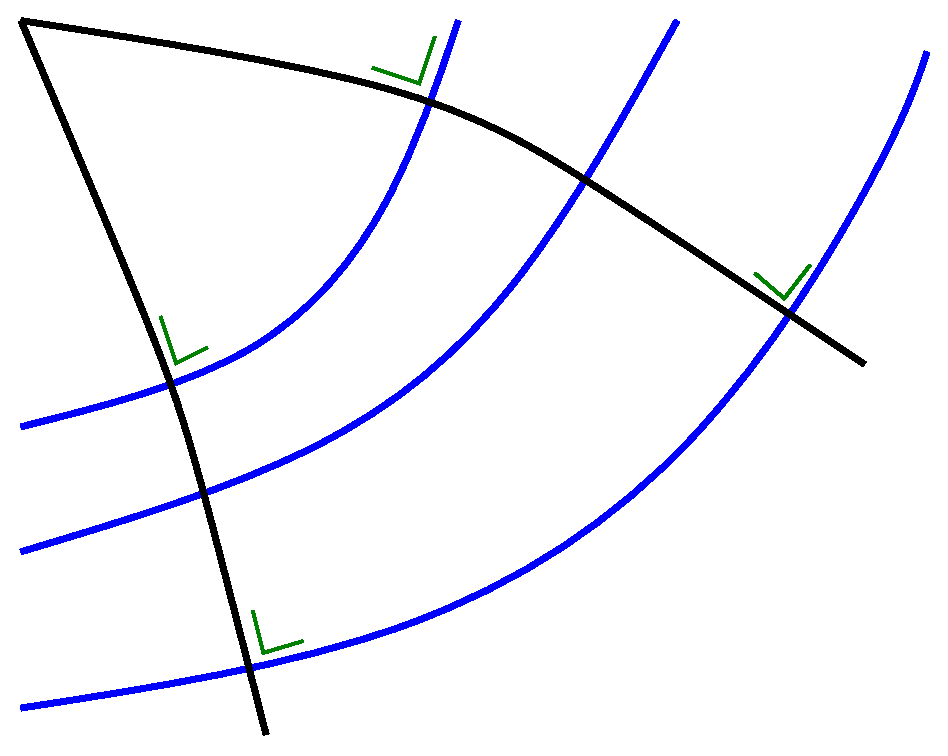
\includegraphics[width=6cm]{figures/RayPath.eps}
\caption{Wave-front (blue) and ray path (black).
}
\label{fig:raypath}
\end{figure}



Note that in the above we used $T({\bf x})=T_0$, where $T_0$ is a
constant, which defines a surface corresponding to a wave front.  This is
the surface corresponding to all parts of the wave which have
travelled a time~$T_0$ since a reference point, usually taken as the
source of the wave.  Ray paths are the lines which are perpendicular
to those surfaces at all points.



We now take the gradient of $\frac{{\rm d}T}{{\rm d}s}=u$ from both sides, we get
\begin{eqnarray}
\frac{{\rm d}\bnabla{T}}{{\rm d}s}=\nabla u\,.
\label{eq_gradv}
\end{eqnarray}
And inserting $\nabla T = U \frac{dr}{ds}$ into $\frac{d{\bf \nabla}T}{ds} = {\bf \nabla} U$ we find
\begin{eqnarray}
\frac{{\rm d}}{{\rm d}s}\left[u \frac{{\rm d} {\bf r}}{{\rm d}s}\right]=\nabla u\,.
\label{eq_ray}
\end{eqnarray}
Knowing the underlying structure of the Earth, implies knowing $u({\bf r})$ and
we can solve (\ref{eq_ray}) for ${\bf r}(s)$ corresponding to the ray followed 
by the wave.

For simplicity we assume that the Earth is radially symmetric and that the 
speed of seismic waves only depends on the radial coordinate $r$ measured from
the centre of the Earth. We actually use the polar coordinates
$(r,\Delta,\phi)$ where we use the letter $\Delta$ instead of the more
common $\theta$ to avoid ambiguity with the wave incident angle. 


% FIG2
\begin{figure}[ht]
    \centering
  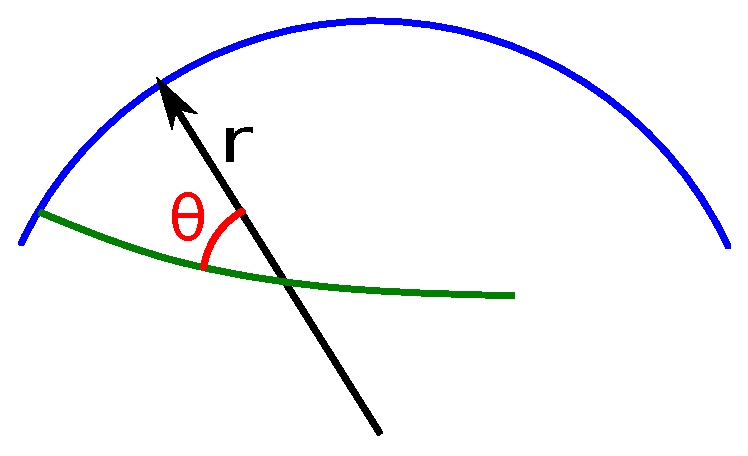
\includegraphics[width=6cm]{figures/rayangle.eps}
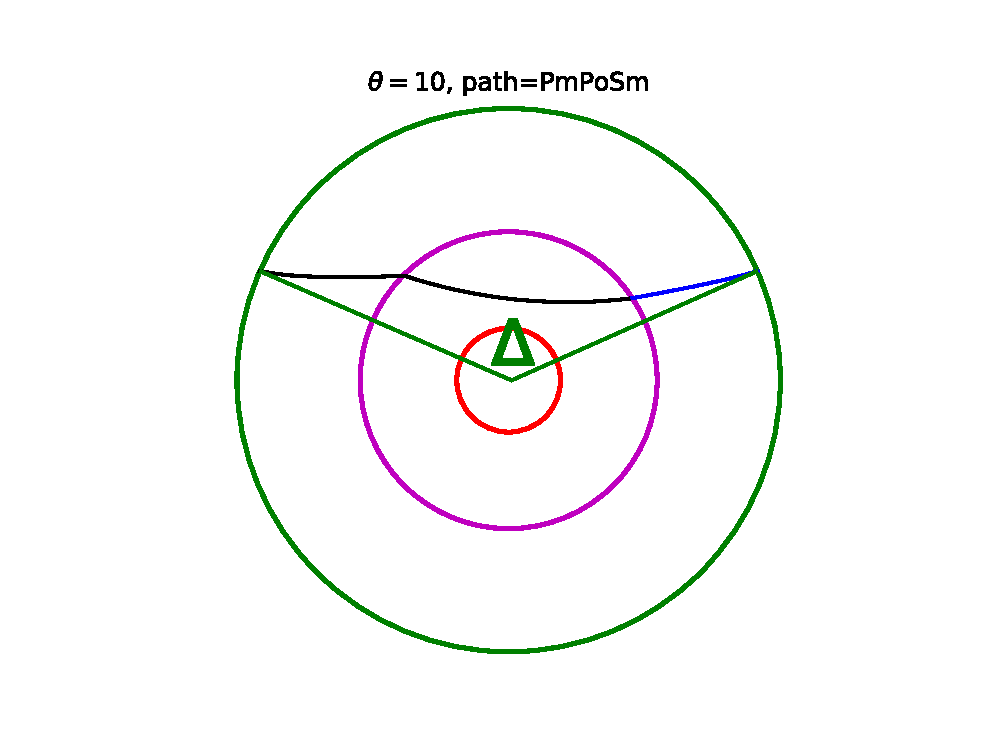
\includegraphics[width=6cm]{figures/demo_trajectory.eps}
\caption{a) Incident angle $\theta$ between ray path (green) and radial 
direction (black).
b) Ray path for a P wave propagating through the mantel and the inner 
core and re-entering the mantel as an S wave (path PmPoSm; the naming
is explained in section~\ref{s:reflection_on_boundary}). $\Delta$ is the 
total deflection angle.}
\label{fig:rayangle}
\end{figure}









\bigskip
\begin{answer}{3}
\begin{eqnarray}
\frac{d}{ds} \left[ {\bf r} \times \left({\bf u} \frac{d{\bf r}}{ds} \right) \right]
\end{eqnarray}
in order to gain the result of this we must use the rule for differentiation over the cross product of two vectors, I shall state this rule below - we are essentially utilising the distributivity of the cross product over differentiation:
\begin{eqnarray}
\left( {\bf u} \times {\bf v} \right)' = \left({\bf u'} \times {\bf v}\right) + \left( {\bf v'} \times {\bf u}\right)
\end{eqnarray}

This is of a similar form to the product rule for differentiation which we are familiar with.

Applying this rule to our example gives the following:
\begin{eqnarray}
\frac{d}{ds} \left[ {\bf r} \times \left({\bf u} \frac{d{\bf r}}{ds} \right) \right] &=& \left( \left(\frac{d{\bf r}}{d {\bf s}} \right) \times \left({\bf u} \frac{d{\bf r}}{d {\bf s}}\right)\right) + \left( {\bf r} \times \left[\frac{d}{d{\bf s}}\left({\bf u}\frac{d {\bf r}}{d {\bf s}} \right) \right]  \right)
\end{eqnarray}

We will in turn analyse each component of the sum of cross products, starting with the following:

\begin{eqnarray}
 \left( \left(\frac{d{\bf r}}{d {\bf s}} \right) \times \left({\bf u} \frac{d{\bf r}}{d {\bf s}}\right)\right) =  {\bf u} \cdot \left( \left(\frac{d{\bf r}}{d {\bf s}} \right) \times \left( \frac{d{\bf r}}{d {\bf s}}\right)\right) = 0
\end{eqnarray}

Here we see the cross product being performed on two identical derivatives, as the two derivatives will have parallel directions it should be clear the cross product will be 0 - as the cross-product essentially produces a vector perpendicular to the plane spanned by the two vectors, as the plane spanned by these two vectors in 3-dimensions is simply a line we know the cross product must be 0. Alternatively, we can use the definition of the cross-product.
 \begin{eqnarray}
 {\bf A}\times {\bf B} = \mid {\bf A}\mid  \cdot \mid {\bf B}\mid  \cdot \sin(\theta)
 \end{eqnarray}
 
so if the result of this is 0, and ${\bf A}$ and ${\bf B}$ are non-zero vectors we know that for the cross-product to be zero then $\sin(\theta) = 0$ - this implies $\Longrightarrow \theta = \{0, \pi, 2\pi, 3\pi, ....\}$ in any case the two vectors are parallel - thus if 2 vectors are parallel their cross product is 0 and vice versa.


 Here we see the cross product of 
\begin{eqnarray}
\left( {\bf r} \times \left[\frac{d}{d{\bf s}}\left({\bf u}\frac{d {\bf r}}{d {\bf s}} \right) \right]  \right)
\end{eqnarray}

This term equates to ${\bf r} \times {\bf \nabla} U$  (refer to above if this is not clear), and since $r$ and ${\bf \nabla U}$ are parallel for a spherically symmetric medium (which we are modelling the Earth as - we can state ${\bf r} \times {\bf \nabla} U = 0$ .

Thus we have shown that 
\begin{eqnarray}
\frac{d}{ds} \left[ {\bf r} \times \left({\bf u} \frac{d{\bf r}}{ds} \right) \right]  = 0
\end{eqnarray}
 Clearly, for a derivative to be 0, the function we have derived must equate to a constant.
\end{answer}

This means that it is preserved along the ray, and its direction is normal to the plane that contains $\frac{dr}{ds}$ and $r$.

We then write
\begin{eqnarray}
\left|{\bf r} \times u \frac{d{\bf r}}{ds}\right|=|{\bf K}| = p = 
r u \sin(\theta_i)
\label{eq_ray4}
\end{eqnarray}


This is because for any vector, we have $\mid a \times b \mid = \mid a \mid \mid b \mid \sin \theta_i$.

where $\theta_i$ is the angle between the ray path 
direction $\frac{d{\bf r}}{ds}$ and the radial direction. 
Notice that $p$, called the ray parameter, is a constant. In other words, 
for any given path, $p$ will remain the same for all times, even when the
wave changes type.

When $\theta_i=\pi/2$, the ray path is 
perpendicular to the radial direction meaning it has reached its lowest point.


We use the eikonal equation in spherical coordinates to evaluate
\begin{equation}
\bnabla T\cdot \bnabla T= \left(\frac{\partial T}{\partial r}\right)^2
+ \frac{1}{r^2} \left(\frac{\partial T}{\partial \theta}\right)^2
+ \frac{1}{r^2\sin(\theta^2)} \left(\frac{\partial T}{\partial \phi}\right)^2
=u({\bf r})^2.
\label{eq_nableTrad}
\end{equation}
For a radially symmetric Earth, waves travel along a great circle and the last 
term is zero. We then seek solution for $T$ of the form 
\begin{eqnarray}
T(r,\theta) = f(\theta)+g(r)
\label{eq_Tansatz}
\end{eqnarray}
and substitute it into (\ref{eq_nableTrad}) to get
\begin{eqnarray}
r^2\left[\frac{d g(r)}{dr}\right]^2-r^2 u(r)^2 = 
-\left[\frac{d f(\theta)}{d\theta}\right]^2 = -k^2.
\label{eq_eikonal2}
\end{eqnarray}
Both sides must be equal to the same constant (explain in your essay why a
constant)
%\marginnote{KP: do the students need to explain it?} 
which we call $-k^2$. 
As $df/d\theta=k$ we have
\begin{eqnarray}
f(\theta) = \int_0^\theta k d\phi = k\theta. 
\label{eq_eikonal_theta}
\end{eqnarray}
From the left hand side of (\ref{eq_eikonal2}) 
\begin{eqnarray}
\frac{d g(r)}{dr}= \pm \left(u(r)^2 -\frac{k^2}{r^2}\right)^{1/2}.
\label{eq_eikonal_g}
\end{eqnarray}
and we have
\begin{eqnarray}
T(r,\theta) = k\theta \pm \int_0^r \left(u(r)^2 -\frac{k^2}{r^2}\right)^{1/2} dr = \left( k\theta \pm \int_{r_s}^r \frac{\sqrt{r^2 u(r)^2 -k^2}}{r} dr \right)
\label{eq_Tansatz2} 
\end{eqnarray}

\begin{answer}{4}
% ANSWER QUESTION 4 HERE

\begin{eqnarray}
\frac{d {\bf r}}{d s} &=&  V \nabla T\\ &=& \frac{\nabla T}{U}
\label{eq_drds} 
\end{eqnarray} 

Here we use the fact that $ V =  \frac{1}{u(r)}$ from our definition of slowness being $U = 1/V$.
The gradient operator $\nabla$ is given by the following for spherical spheres $\nabla = \left[ \frac{\partial}{\partial r}, \frac{1}{r}\frac{\partial}{\partial \theta}, \frac{1}{r\sin \theta}\frac{\partial}{\partial \theta} \right]$.

Using this in our equation gives the following:
\begin{eqnarray}
\frac{d {\bf r}}{d s} &=&  V \nabla T\\ &=& \frac{\nabla T}{U}\\ &=& \frac{1}{U}\left[\frac{\partial T}{\partial r}, \frac{1}{r}\frac{\partial T}{\partial \theta}, \frac{1}{r\sin \theta}\frac{\partial T}{\partial \theta}\right]
\label{eq_drds} 
\end{eqnarray}
From:
\begin{eqnarray}
T(r,\theta) = k\theta \pm \int_0^r \left(u(x)^2 -\frac{k^2}{x^2}\right)^{1/2} dx.
\label{eq_Tansatz2} 
\end{eqnarray}
we know that this can be substituted in to give the following:
\begin{eqnarray}
\frac{d {\bf r}}{d s} &=& \frac{1}{U}\left[\frac{\partial T}{\partial r}, \frac{1}{r}\frac{\partial T}{\partial \theta}, \frac{1}{r\sin \theta}\frac{\partial T}{\partial \theta}\right]\\
&=&  \frac{1}{U}\left[\frac{\partial}{\partial r} \left( k\theta \pm \int_{r_s}^r \frac{\sqrt{r^2 u(r)^2 -k^2}}{r} dr \right), \frac{1}{r}\frac{\partial}{\partial \theta}  \left( ... \right), \frac{1}{r\sin \theta}\frac{\partial}{\partial \theta} \left( ... \right)\right]\\ &=&  \frac{1}{U}\left[ \pm \frac{\sqrt{r^2 u(r)^2 -k^2}}{r}, \frac{k}{r}, 0\right]
\label{eq_drds} 
\end{eqnarray} 
Hint: search the literature to find the expression for the gradient 
($\bnabla$) in polar coordinates.
\end{answer}

As $|d {\bf r}/d s|=1$, the angle $\theta$ between the incident 
ray path and the radial direction is
\begin{eqnarray} 
\sin(\theta) = \frac{k}{r u(r)} 
\end{eqnarray}
and so $k=r u(r) \sin(\theta) = p$ (see (\ref{eq_ray4})). 
Then $T(r,\theta)$ can be obtained by computing the integral
\begin{eqnarray}
T(r,\theta) = p\theta \pm \int_{r_s}^r \frac{\sqrt{x^2 u(x)^2 -p^2}}{x} dx.
\label{eq_Ta} 
\end{eqnarray}
with $r_s$ the radius at the starting point. As $T$ is a travelling time it 
must increase and so we take the $+$ sign for ascending waves, $dr>0$, and
the $-$ sign for descending waves, $dr <0$. 

It can be shown \cite{Rawlinson} that the wave travelling time along the 
path is a local minimum (Fermat's principle).
Mathematically:
\begin{eqnarray}
\frac{\partial T}{\partial p} =  \theta \pm 
\int_{r_s}^r \frac{-p}{x\sqrt{r^2 u(x)^2 - p^2}} dx=0
\label{eq_dTdp} 
\end{eqnarray} 
and so
\begin{eqnarray}
\theta = \pm p
\int_{r_s}^r \frac{1}{x\sqrt{r^2 u(x)^2 - p^2}} dx.
\label{eq_theta} 
\end{eqnarray} 
Substituting this back into (\ref{eq_Ta}):
\begin{eqnarray}
T(r,\theta) &=&\pm \int_{r_s}^{r}\left[  \frac{p^2}{x\sqrt{x^2 u(x)^2 - p^2}} +
  \frac{\sqrt{x^2 u(x)^2 -p^2}}{x} \right]dx\\
&=&\pm \int_{r_s}^{r}  \frac{x^2u(x)^2}{x\sqrt{x^2 u(x)^2 - p^2}} dx
\label{eq_Tb} 
\end{eqnarray}

The total angle of propagation between 2 points can be determined from 
(\ref{eq_theta}):
\begin{eqnarray}
\Delta = \int_{r_s}^{r} \frac{p}{x\sqrt{x^2u(x)^2 - p^2}} dx.
\label{eq_delta} 
\end{eqnarray} 


\begin{answer}{5}
% ANSWER QUESTION 5 HERE
In order to gain an accurate approximation of the time that a Seismic wave (earthquake) in one place is likely to affect another place we can do the following (using the examples of Durham and Tokyo as locations).
Initially I approximated the angle (from the centre of the earth between the two locations).
I used the bearing of Durham ($+54.7754^{\circ} N$  and $-1.5849^{\circ} W$ and the for Tokyo ($+35.6895^{\circ} N$  and $139.6917^{\circ} E$.

As we have the bearings of the individual angles, we can use them and the following formula to calculate the Central Subtended Angle between the two locations.

\begin{eqnarray}
\alpha = \cos^-1 \left( \sin \phi_1 \sin \phi_2 + \cos \phi_1 \cos \phi_2 \cos \Delta \lambda \right)
\end{eqnarray} 

Here we use $\phi$ as the latitude angles and $\Delta \lambda$ as the difference between the longitude angles, subtituing the appropriate values in gives:

\begin{eqnarray}
\alpha &=& \cos^-1 \left( \sin (54.7753) \sin (36.6895) + \cos (54.7753) \cos (36.6895) \cos (141.2766) \right)\\
&=& 83.62177876^{\circ}
\end{eqnarray} 

In order to confirm this is approximately the right angle using it to calculate the great circle distance between Durham and Tokyo gives us $\sigma = 2\pi r_E \frac{\alpha}{360} = 9298.31755$ which is approximately the great circle distance between Durham, where we used $r_E$ as the average radius of the Earth - approximately 6371km.

We can run our program modelling the wave with different values of $\theta$, and when the value of $\delta$ is approximately $83.62177876^{\circ}$ we will assume the value of T to be a reasonable approximation of the time it takes.


\begin{center}
\begin{tabular}{ |c|c|c|c| } 
 \hline
 ${\bf \theta}$ & Wave Type & ${\bf T}$ & ${\bf \delta}$\\
 15 & Primary & 759.9334 & 85.5325 \\ 
 17.5 & Primary & 702.3417 & 74.8416 \\ 
 16.75 & Primary & 723.0295 & 78.5003 \\ 
 15.875 & Primary & 741.6731 & 81.9617 \\ 
 16.0 & Primary & 741.7797 & 81.9807 \\
 16.5 & Primary & 727.8186 & 79.3735\\ 
 \hline
\end{tabular}
\end{center}

Thus the approximate time for a Primary wave to travel from Durham to Tokyo is around 741.7797 seconds - as this is at the angle $16.0^{\circ}$ which corresponds to an angle $\delta$ and is the closest approximation ( to the nearest 0.5 degrees) to the actual central subtended angle that we calculated.

\begin{center}
\begin{tabular}{ |c|c|c|c| } 
 \hline
 ${\bf \theta}$ & Wave Type & ${\bf T}$ & ${\bf \delta}$\\
 15 & Secondary & 1525.1960 & 100.2501 \\ 
 20 & Secondary & 1262.1571 & 73.1535 \\ 
 17.5 & Secondary & 1382.9630 & 84.4846 \\ 
 18.75 & Secondary & 1325.0099 & 78.8622 \\ 
 18.5 & Secondary & 1334.7707 & 79.78197 \\
 18.0 & Secondary & 1361.1517 & 82.3224\\ 
 \hline
\end{tabular}
\end{center}

Thus the approximate time for a Secondary wave to travel from Durham to Tokyo is around 1382.9630 seconds - as this is at the angle $17.5^{\circ}$ which corresponds to an angle $\delta$ and is the closest approximation ( to the nearest 0.5 degrees) to the actual central subtended angle that we calculated.

\end{answer}

\begin{answer}{6}
% ANSWER QUESTION 6 HERE
\end{answer}

\section{Conclusions}
Yet to write a conclusion, apologies - also yet to incorporate my python code into my essay as answered questions first and wasn't able to finish the essay in time, any feedback on what I have produced would be appreciated.

\begin{thebibliography}{99}

\bibitem{Rawlinson}
Nick rawlinson {\it Lecture notes on Seismology}
\url{http://rses.anu.edu.au/~nick/teaching.html}

\bibitem{EarthModel}
Adam M. Dziewonski and Don L. Anderson
{\it Preliminary reference Earth model}
Physics of the Earth and Planetary Interiors, 25 (1981) 297—356

\bibitem{PREM}
Peter Bormann
{\it Global 1-D Earth models}
DOI: \url{http://doi.org/10.2312/GFZ.NMSOP_r1_DS_2.1}


\end{thebibliography}
\end{document}
